%%%%%%%%%%%%%%%%%%%%%%%%%%%%%%%%%%%%%%%%%%%%%%%%%%%%%%%%%%%%%%%%%
% MUW Presentation
% LaTeX Template
% Version 1.0 (27/12/2016)
%
% License:
% CC BY-NC-SA 4.0 (http://creativecommons.org/licenses/by-nc-sa/3.0/)
%
% Created by:
% Nicolas Ballarini, CeMSIIS, Medical University of Vienna
% nicoballarini@gmail.com
% http://statistics.msi.meduniwien.ac.at/
%
% Customized for UAH by:
% David F. Barrero, Departamento de Automática, UAH
%%%%%%%%%%%%%%%%%%%%%%%%%%%%%%%%%%%%%%%%%%%%%%%%%%%%%%%%%%%%%%%%%

\documentclass[10pt,compress]{beamer} % Change 10pt to make fonts of a different size
\mode<presentation>

\usepackage[spanish]{babel}
\usepackage{fontspec}
\usepackage{tikz}
\usepackage{etoolbox}
\usepackage{xcolor}
\usepackage{xstring}
\usepackage{listings}
\usepackage{tikz}
\usetikzlibrary{matrix,chains,positioning,decorations.pathreplacing,arrows,shapes}
\usepackage{pgf-umlcd} % Soporte para diagramas UML con Tikz
\usepackage{multicol}

\usetheme{UAH}
\usecolortheme{UAH}
\setbeamertemplate{navigation symbols}{} 
\setbeamertemplate{caption}[numbered]

%%%%%%%%%%%%%%%%%%%%%%%%%%%%%%%%%%%%%%%%%%%%%%%%%%%%%%%%%%%%%%%%%
%% Presentation Info
\title{OOP in Arcade}
\author{\asignatura\\\carrera}
\institute{}
\date{Departamento de Automática}
%%%%%%%%%%%%%%%%%%%%%%%%%%%%%%%%%%%%%%%%%%%%%%%%%%%%%%%%%%%%%%%%%


%%%%%%%%%%%%%%%%%%%%%%%%%%%%%%%%%%%%%%%%%%%%%%%%%%%%%%%%%%%%%%%%%
%% Descomentar para habilitar barra de navegación superior
\setNavigation
%%%%%%%%%%%%%%%%%%%%%%%%%%%%%%%%%%%%%%%%%%%%%%%%%%%%%%%%%%%%%%%%%

%%%%%%%%%%%%%%%%%%%%%%%%%%%%%%%%%%%%%%%%%%%%%%%%%%%%%%%%%%%%%%%%%
%% Configuración de logotipos en portada
%% Opacidad de los logotipos
\newcommand{\opacidad}{1}
%% Descomentar para habilitar logotipo en pié de página de portada
%\renewcommand{\logoUno}{Images/isg.png}
%% Descomentar para habilitar logotipo en pié de página de portada
%\renewcommand{\logoDos}{Images/CCLogo.png}
%% Descomentar para habilitar logotipo en pié de página de portada
\renewcommand{\logoTres}{Images/ALogo.png}
%% Descomentar para habilitar logotipo en pié de página de portada
%\renewcommand{\logoCuatro}{Images/ELogo.png}
%%%%%%%%%%%%%%%%%%%%%%%%%%%%%%%%%%%%%%%%%%%%%%%%%%%%%%%%%%%%%%%%%

%%%%%%%%%%%%%%%%%%%%%%%%%%%%%%%%%%%%%%%%%%%%%%%%%%%%%%%%%%%%%%%%%
%% FOOTLINE
%% Comment/Uncomment the following blocks to modify the footline
%% content in the body slides. 


%% Option A: Title and institute
\footlineA
%% Option B: Author and institute
%\footlineB
%% Option C: Title, Author and institute
%\footlineC
%%%%%%%%%%%%%%%%%%%%%%%%%%%%%%%%%%%%%%%%%%%%%%%%%%%%%%%%%%%%%%%%%

\begin{document}

%%%%%%%%%%%%%%%%%%%%%%%%%%%%%%%%%%%%%%%%%%%%%%%%%%%%%%%%%%%%%%%%%
% Use this block for a blue title slide with modified footline
{\titlepageBlue
    \begin{frame}
        \titlepage
    \end{frame}
}

\institute{\asignatura}

\begin{frame}[plain]{}
	\begin{block}{Objectives}
		\begin{enumerate}
		\item Understand the OO API in Arcade
		\item Use sprites and sprites sheets with Arcade
		\item Handle user input
		\item Understand some multimedia file formats
		\item Introduce the \texttt{Window}, \texttt{View} and \texttt{Sprite} classes
		\end{enumerate}
	\end{block}

   	\begin{block}{Bibliography}
      		\begin{enumerate}
			\item Paul Craven. \textit{The Arcade Book. Chapter 18: Using the Window class}. \href{https://learn.arcade.academy/en/latest/chapters/18\_window\_class/window\_class.html}{(link)}.
			\item Paul Craven. \textit{The Arcade Book. Chapter 19: User control}. \href{https://learn.arcade.academy/en/latest/chapters/18\_window\_class/window\_class.html}{(link)}.
			\item Paul Craven. \textit{The Arcade Book. Chapter 21: Spriters and collisions}. \href{https://learn.arcade.academy/en/latest/chapters/21\_sprites\_and\\_collisions/sprites.html}{(link)}.
			\item Paul Craven. \textit{Using Views for Start/End Screens}. \href{https://api.arcade.academy/en/stable/tutorials/views/index.html}{(link)}.
      		\end{enumerate} 
   	\end{block}
\end{frame}

{
\disableNavigation{white}
\begin{frame}[shrink]{Table of Contents}

 	\frametitle{Table of Contents}
  	\begin{multicols}{2}
  		\tableofcontents
    \end{multicols}

 %\frametitle{Table of Contents}
 %\tableofcontents
  % You might wish to add the option [pausesections]
\end{frame}
}

\section{The Window class}
\subsection{Introduction}

\begin{frame}{The \texttt{Window} class}{Introduction}
	Arcade has an OOP API
	\begin{itemize}
		\item More features than structured API
		\item Easy to use API
	\end{itemize}
\end{frame}

\begin{frame}{The \texttt{Window} class}{Introduction (II)}
	\begin{exampleblock}{}
		\vspace{-0.2cm}
		\lstinputlisting[numbers=left]{code/window.py}
		\vspace{-0.2cm}
	\end{exampleblock}
\end{frame}

\begin{frame}{The \texttt{Window} class}{Introduction (III)}
	\begin{exampleblock}{}
		\vspace{-0.2cm}
		\lstinputlisting[numbers=left]{code/window-main.py}
		\vspace{-0.2cm}
	\end{exampleblock}
\end{frame}

\subsection{Basic methods}

\begin{frame}{The \texttt{Window} class}{Constructor}
	\begin{block}{Constructor}
		\vspace{-0.2cm}
		\lstinputlisting{code/window-init.py}
		\vspace{-0.2cm}
	\end{block}	

    Remember to use reference documentation
	\begin{itemize}
		\item \href{https://api.arcade.academy/en/2.6.17/api/window.html\#arcade.Window}{(\texttt{arcade.Window} reference)}
        \item $\frac{1}{0.016666666666666666} = 60 Hz$
        \item Antialiasing: Smoothing transitions between colors and shapes
	\end{itemize}

\end{frame}

\subsection{Main methods and attributes}
\begin{frame}{The \texttt{Window} class}{Main methods and attributes}
	\begin{block}{\texttt{arcade.Window}}
		\smallskip
		\begin{columns}[t]
 	   \column{.5\textwidth}
			\centering \textbf{Methods}
		\begin{itemize}
		\item \footnotesize{\texttt{setup()}}. \\Initialization
		\item \footnotesize{\texttt{on\_draw()}}. \\Drawing
		\item \footnotesize{\texttt{on\_update(delta\_time: float)}}. \\Move everything. Perform collision checks. Do all the game logic here
		\end{itemize}

 	   \column{.5\textwidth}
		\centering \textbf{Attributes}
		\begin{itemize}
		\item \footnotesize{\texttt{background\_color}}.
		\end{itemize}
    	\end{columns}
	\end{block}	
\end{frame}

\subsection{Background}

\begin{frame}{The \texttt{Window} class}{Background (I)}
    \begin{exampleblock}{}
	\vspace{-0.2cm}
	\lstinputlisting[numbers=left]{code/background-1.py}
	\vspace{-0.2cm}
    \end{exampleblock}

    \centering \href{https://api.arcade.academy/en/latest/arcade.color.html}{(List of colors)}

    \bigskip

    \begin{columns}
 	   \column{.7\textwidth}
		\begin{exampleblock}{}
		\vspace{-0.2cm}
		\lstinputlisting[numbers=left]{code/background-2.py}
		\vspace{-0.2cm}
		\end{exampleblock}

 	   \column{.3\textwidth}
		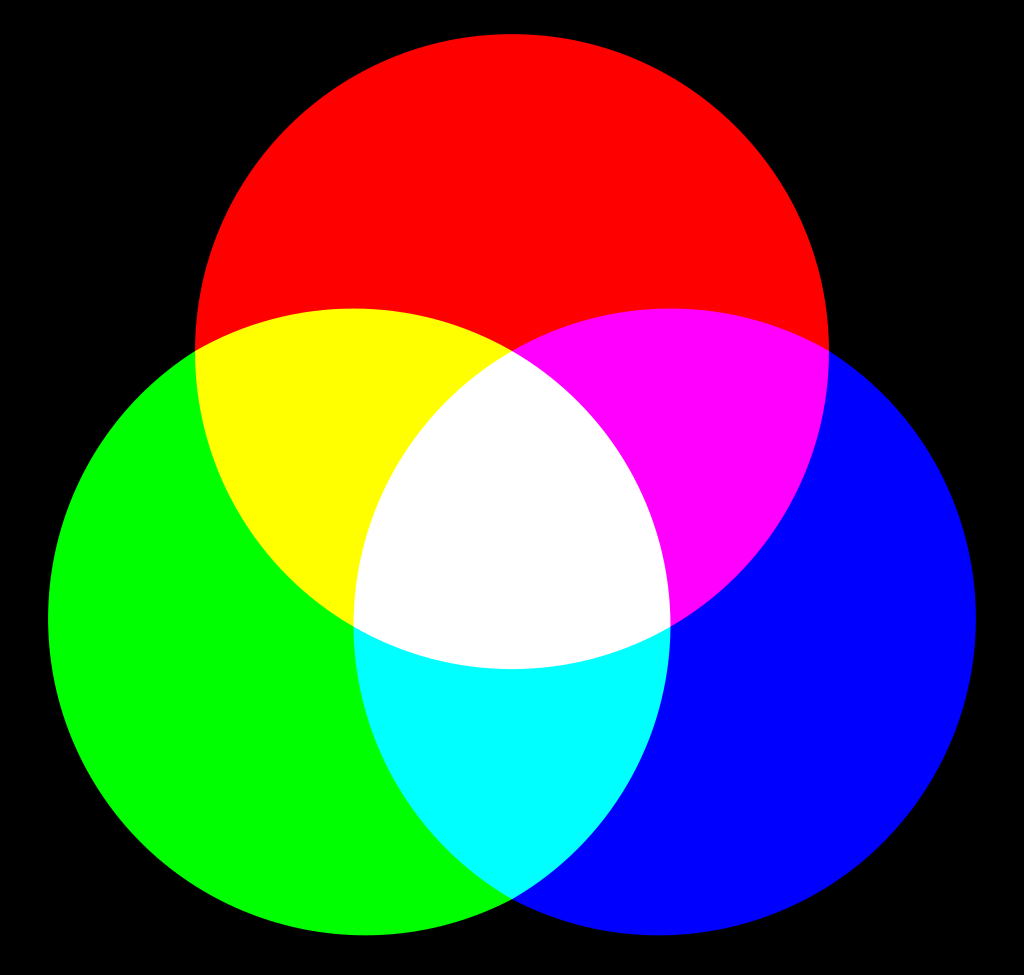
\includegraphics[width=\linewidth]{figs/rgb}\\
    \end{columns}
\end{frame}

\begin{frame}[plain]{The \texttt{Window} class}{Background (II)}
	\centering 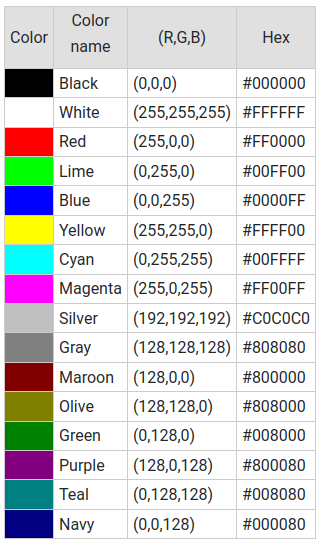
\includegraphics[width=0.4\linewidth]{figs/colors}\\
	\tiny \href{https://www.rapidtables.com/convert/color/rgb-to-hex.html}{(Source)}
\end{frame}

\subsection{User control methods}

\begin{frame}{The \texttt{Window} class}{User control methods (I)}
	\begin{block}{User control methods}
	%	\vspace{-0.15cm}
		\begin{itemize}
		\item \footnotesize{\texttt{on\_key\_press(key)}} Called when the user presses key.
		\item \footnotesize{\texttt{on\_key\_release(symbol: int, modifiers: int)}}. Called when the user presses key.
		\item \footnotesize{\texttt{on\_mouse\_press(x: float, y: float, button: int, modifiers: int)}}. Called when the user presses a mouse button.
		\item \footnotesize{\texttt{on\_mouse\_release(x: float, y: float, button: int, modifiers: int)}}.  Called when the user releases a mouse button.
		\item \footnotesize{\texttt{on\_mouse\_motion(x, y, delta\_x, delta\_y)}}. Called whenever the mouse moves.
		\end{itemize}
	%	\vspace{-0.2cm}
	\end{block}	
\end{frame}

\begin{frame}[plain]{The \texttt{Window} class}{User control methods: Examples}
	\begin{exampleblock}{Capturing a key}
		\vspace{-0.2cm}
		\lstinputlisting[numbers=left]{code/key.py}
		\vspace{-0.2cm}
	\end{exampleblock}

	\begin{exampleblock}{Capturing a mouse click}
		\vspace{-0.2cm}
		\lstinputlisting[numbers=left]{code/button.py}
		\vspace{-0.2cm}
	\end{exampleblock}

	\href{https://api.arcade.academy/en/2.6.17/arcade.key.html}{(More info about keys)}
\end{frame}

\subsection{Other methods}

\begin{frame}{The \texttt{Window} class}{Other methods}
	\begin{block}{Other methods}
	%	\vspace{-0.15cm}
		\begin{itemize}
		\item \footnotesize{\texttt{activate()}}. 
		\item \footnotesize{\texttt{center\_window()}}. 
		\item \footnotesize{\texttt{close()}}. 
		\item \footnotesize{\texttt{get\_location()}}. 
		\item \footnotesize{\texttt{maximize()} and \texttt{minimize()}}. 
		\item \footnotesize{\texttt{set\_fullscreen(fullscreen: bool = True)}}. 
		\item \footnotesize{\texttt{set\_location(x, y)}}. 
		\item \footnotesize{\texttt{set\_viewport(left: float, right: float, bottom: float, top: float)}}. Set the coordinates we can see
		\end{itemize}
	%	\vspace{-0.2cm}
	\end{block}	
\end{frame}

\section{Using a game controller}

\begin{frame}{The \texttt{Window} class}{Using a game controller (I)}
	First, get the controllers with \texttt{arcade.get\_joysticks()}
	\begin{exampleblock}{Get game controllers}
		\vspace{-0.2cm}
		\lstinputlisting[numbers=left]{code/joystick-get.py}
		\vspace{-0.2cm}
	\end{exampleblock}

	\begin{exampleblock}{Read game controller value}
		\vspace{-0.2cm}
		\lstinputlisting[numbers=left]{code/joystick-value.py}
		\vspace{-0.2cm}
	\end{exampleblock}	
\end{frame}

\begin{frame}{The \texttt{Window} class}{Using a game controller (II)}
	\begin{exampleblock}{Read game controller value}
	\vspace{-0.2cm}
	\lstinputlisting[numbers=left]{code/joystick-value.py}
	\vspace{-0.2cm}
	\end{exampleblock}	

	\bigskip

    \begin{columns}
 	   \column{.25\textwidth}
		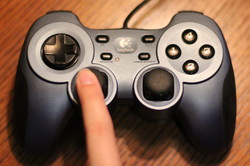
\includegraphics[width=\linewidth]{figs/controller-centered.jpg}\\
		\centering Centered $(0,0)$
	   \column{.25\textwidth}
		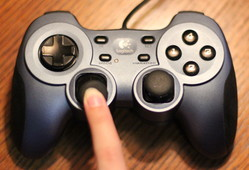
\includegraphics[width=\linewidth]{figs/controller-down.jpg}\\
		\centering Down $(0,1)$
	   \column{.25\textwidth}
		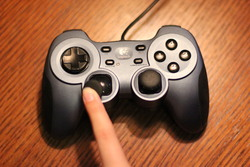
\includegraphics[width=\linewidth]{figs/controller-downleft.jpg}\\
		\centering Down-left $(-1, 1)$
 	   \column{.25\textwidth}
		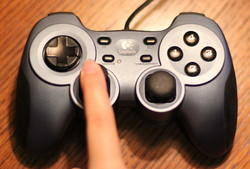
\includegraphics[width=\linewidth]{figs/controller-up.jpg}\\
		\centering Up $(0,-1)$
    \end{columns}

	\centering \tiny \href{https://learn.arcade.academy/en/latest/chapters/19\_user\_control/user\_control.html}{(Source)}

	\bigskip

	\normalsize
	\href{https://api.arcade.academy/en/2.6.17/examples/sprite\_move\_joystick.html}{(Interesting example)}

\end{frame}

\section{Life-cycle management}

\subsection{Graphs}

\begin{frame}{Life-cycle management}{Graphs}
	\begin{columns}
 	   \column{.50\textwidth}
		\alert{Graph}: Data structure with \textbf{nodes} and \textbf{edges}

		\begin{itemize}
		\item Widely used in programming, AI and videogames
		\item Huge number of applications
		\end{itemize}

		Central role in \alert{path planning}
		\begin{itemize}
		\item \href{https://www.youtube.com/watch?v=tH9dNESH4ic}{(Video)}
		\item Navigation mesh
		\end{itemize}

 	   \column{.50\textwidth}
	   	\begin{tikzpicture}[scale=0.5]
		\tikzstyle{node_style} = [circle,draw=black]
	    	\tikzstyle{edge_style} = [draw=black]
		\node[node_style] (v1) at (-2,2) {2};
		\node[node_style] (v2) at (2,2) {3};
		\node[node_style] (v3) at (4,0) {6};
		\node[node_style] (v4) at (2,-2) {4};
		\node[node_style] (v5) at (-2,-2) {5};
		\node[node_style] (v6) at (-4,0) {1};
		\draw[edge_style] (v1) edge (v2);
		\draw[edge_style] (v2) edge (v3);
		\draw[edge_style] (v3) edge (v4);
		\draw[edge_style] (v4) edge (v5);
		\draw[edge_style] (v5) edge (v6);
		\draw[edge_style] (v6) edge (v1);
		\draw[edge_style] (v5) edge (v1);
		\draw[edge_style] (v5) edge (v2);
		\draw[edge_style] (v4) edge (v2);
	    	\end{tikzpicture}
    \end{columns}
\end{frame}

\subsection{Finite States Machines}

\begin{frame}{Life-cycle management}{Finite States Machines (I)}
	\begin{columns}
 	  \column{.50\textwidth}
		\begin{block}{Finite-State Machine (FSM)}
	    	A graph whose nodes represent states, usually associated with behaviours
		\end{block}
	\end{columns}

	\bigskip

	\begin{columns}
 	   \column{.20\textwidth}
		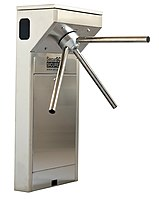
\includegraphics[width=\linewidth]{figs/turnstile}\\
 	   \column{.50\textwidth}
		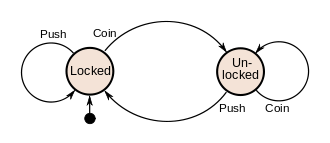
\includegraphics[width=\linewidth]{figs/fsm}\\
		\centering \tiny \href{https://en.wikipedia.org/wiki/Finite-state\_machine}{(Source)}
	\end{columns}
\end{frame}

\begin{frame}{Life-cycle management}{Finite States Machines (II)}
	FSMs have many applications
	    \begin{itemize}
	    \item Central role in Theory of Computation
	    \item Good to model behaviours ... such as a NPC or an entire videogame
	    \end{itemize}

	\bigskip

	\begin{columns}
 	   \column{.5\textwidth}
		\centering NPC behaviour\\
		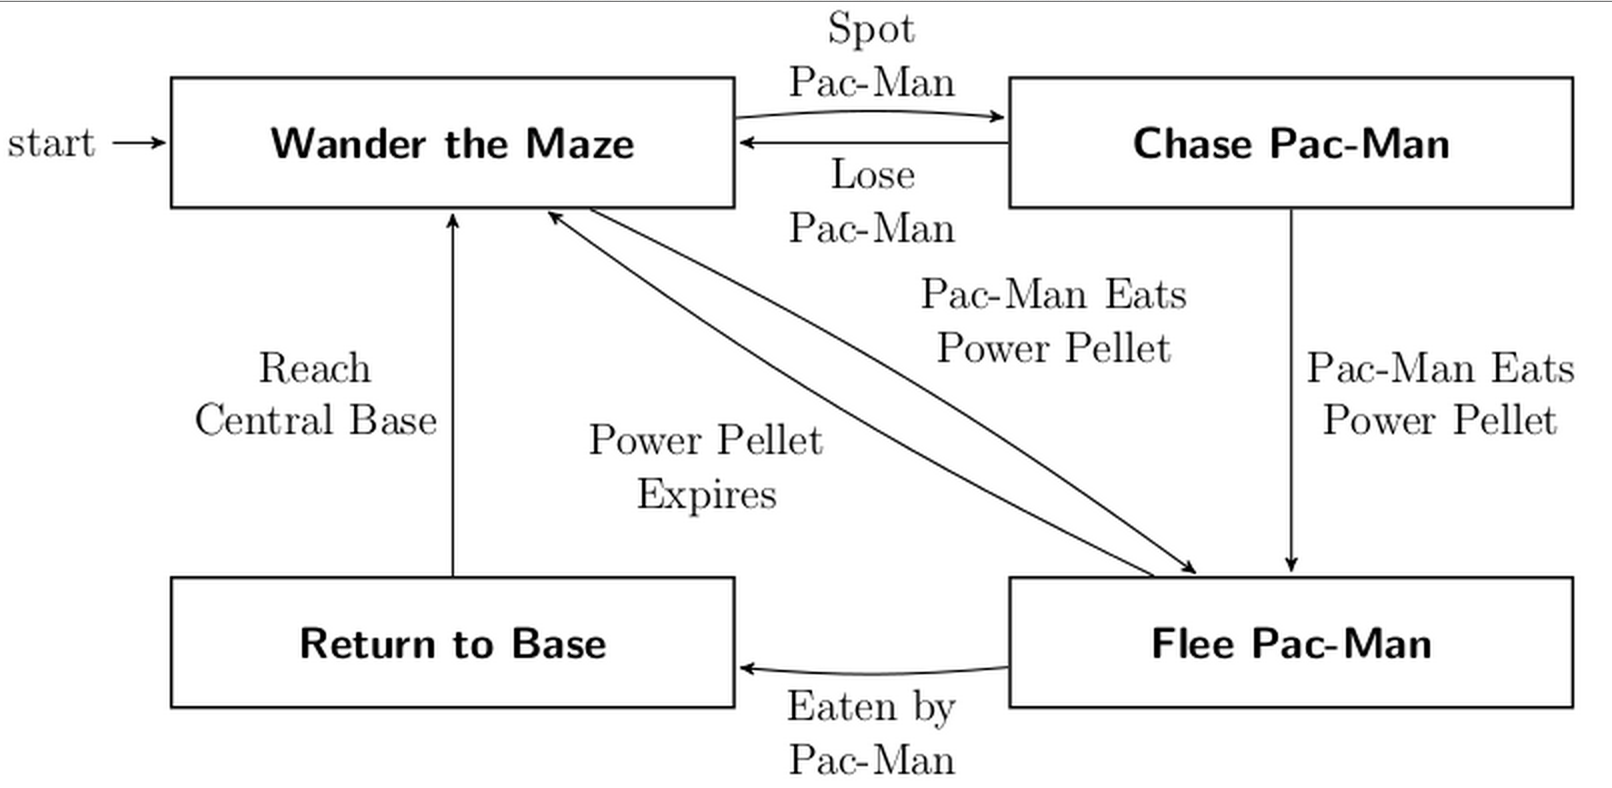
\includegraphics[width=\linewidth]{figs/fsm-pacman.png}\\
		\centering \tiny \href{http://bits.citrusbyte.com/state-design-pattern-with-ruby/}{(Source)}
 	   \column{.5\textwidth}
		\centering Game life-cycle (also state) \\
		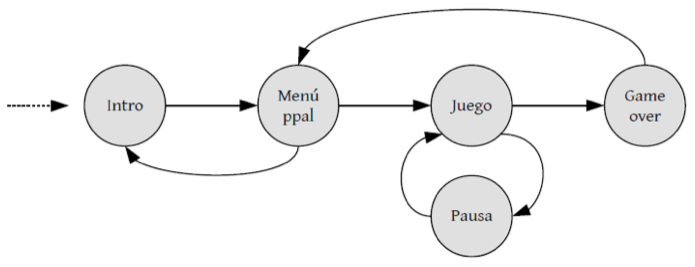
\includegraphics[width=\linewidth]{figs/states}\\
	\end{columns}
\end{frame}


\subsection{The View class}

\begin{frame}{Life-cycle management}{The \texttt{View} class (I)}
	Videogames use several screens, or states
	\begin{itemize}
    		\item Start screens
    		\item Instruction screens
    		\item Game over screens
    		\item Pause screens
	\end{itemize}

	Arcade provides the \texttt{View} class
	\begin{itemize}
		\item Very much like the Window class
		\item It has the \texttt{on\_draw()} and \texttt{on\_update()} methods
	\end{itemize}


	\vspace{-3.5cm}
    \hfill 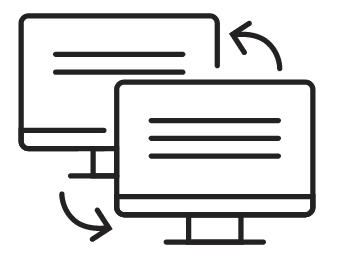
\includegraphics[width=0.3\linewidth]{figs/screens.png}
	\tiny  \href{https://api.arcade.academy/en/stable/tutorials/views/index.html}{(Source)}
\end{frame}

\begin{frame}{Life-cycle management}{The \texttt{View} class (II)}
	Our class must derive from \texttt{arcade.View}
	\begin{columns}
 	   %\column{.1\textwidth}
 	   \column{.4\textwidth}
		\begin{exampleblock}{}
		\lstinline{class MyGame(arcade.Window):}
		\end{exampleblock}
 	   \column{.1\textwidth}
		$\Rightarrow$
 	   \column{.35\textwidth}
		\begin{exampleblock}{}
		\lstinline{class MyGame(arcade.View):}
		\end{exampleblock}
 	   \column{.05\textwidth}
	\end{columns}

	\bigskip

	The view does not control the window size, so
	\begin{columns}
 	   %\column{.1\textwidth}
 	   \column{.4\textwidth}
		\begin{exampleblock}{}
		\lstinline{super().__init__(SCREEN_WIDTH, SCREEN_HEIGHT, SCREEN_TITLE)}
		\end{exampleblock}
 	   \column{.1\textwidth}
		$\Rightarrow$
 	   \column{.3\textwidth}
		\begin{exampleblock}{}
		\lstinline{super().__init__()}
		\end{exampleblock}
 	   \column{.1\textwidth}
	\end{columns}
\end{frame}

\begin{frame}[fragile]{Life-cycle management}{The \texttt{View} class (III)}
	Finally, we need to create a window, a view and show that view
	\begin{columns}
 	   %\column{.1\textwidth}
 	   \column{\textwidth}
		\begin{exampleblock}{}
			\begin{lstlisting} 
def main():
    """ Main function """

    window = arcade.Window(SCREEN_WIDTH, SCREEN_HEIGHT, SCREEN_TITLE)
    start_view = GameView()
    window.show_view(start_view)
    start_view.setup()
    arcade.run()
\end{lstlisting}
		\end{exampleblock}
	\end{columns}
\end{frame}

\subsection{The View class: Example}

\begin{frame}[fragile]{Life-cycle management}{The \texttt{View} class: Example (I)}
		\begin{exampleblock}{GameOverView view}
			\begin{lstlisting}[numbers=left]
class GameOverView(arcade.View):
    """ View to show when game is over """

    [...]

    def on_draw(self):
        """ Draw this view """
        self.clear()
        self.texture.draw_sized(SCREEN_WIDTH / 2, SCREEN_HEIGHT / 2, SCREEN_WIDTH, SCREEN_HEIGHT)

    def on_mouse_press(self, _x, _y, _button, _modifiers):
        """ If the user presses the mouse button, re-start the game. """
        game_view = GameView()
        game_view.setup()
        self.window.show_view(game_view)
\end{lstlisting}
\end{exampleblock}
\end{frame}

\begin{frame}[fragile]{Life-cycle management}{The \texttt{View} class: Example (II)}
		\begin{exampleblock}{Game view}
			\begin{lstlisting}[numbers=left]
def on_update(self, delta_time):
        """ Movement and game logic """

        [ ... ]

        # Check length of coin list. If it is zero, flip to the
        # game over view.
        if len(self.coin_list) == 0:
            view = GameOverView()
            self.window.show_view(view)
\end{lstlisting}
\end{exampleblock}
\end{frame}

\section{Sprites}
\subsection{Introduction}

\begin{frame}{Sprites}{Introduction}
    \begin{columns}
 	   \column{.50\textwidth}
	   \begin{block}{Sprite}
       A sprite is a 2D image used in videogames
	   \end{block}
   \end{columns}

    \bigskip

    \begin{columns}
 	   \column{.20\textwidth}
			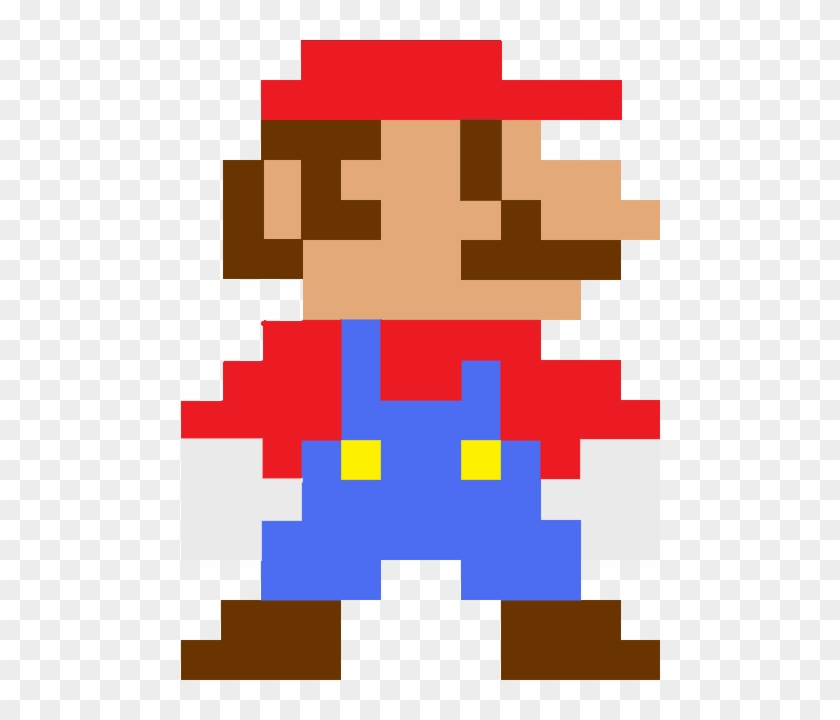
\includegraphics[width=\linewidth]{figs/mario.jpg}\\
 	   \column{.20\textwidth}
			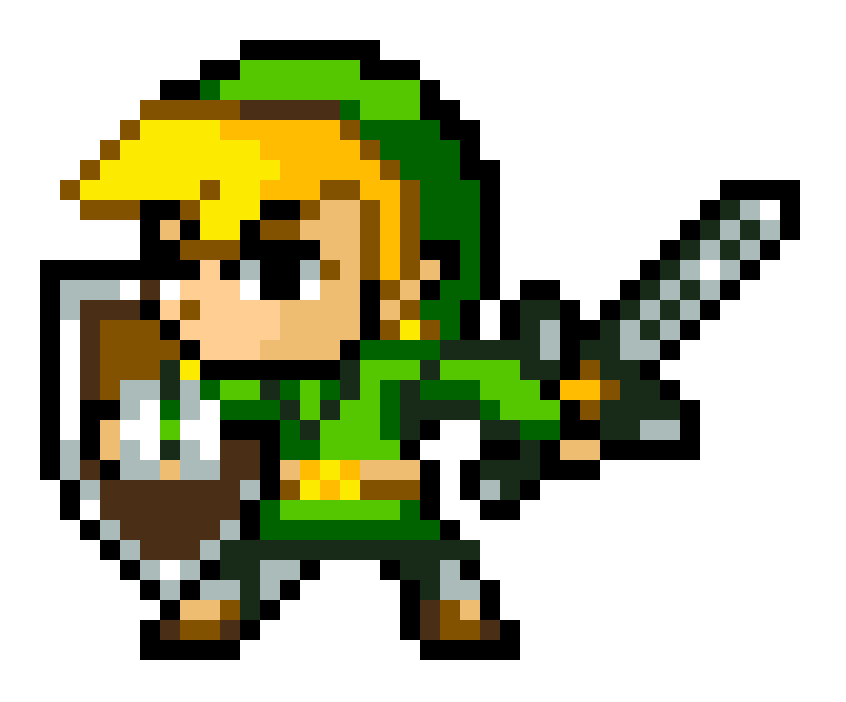
\includegraphics[width=\linewidth]{figs/zelda.png}\\
 	   \column{.50\textwidth}
			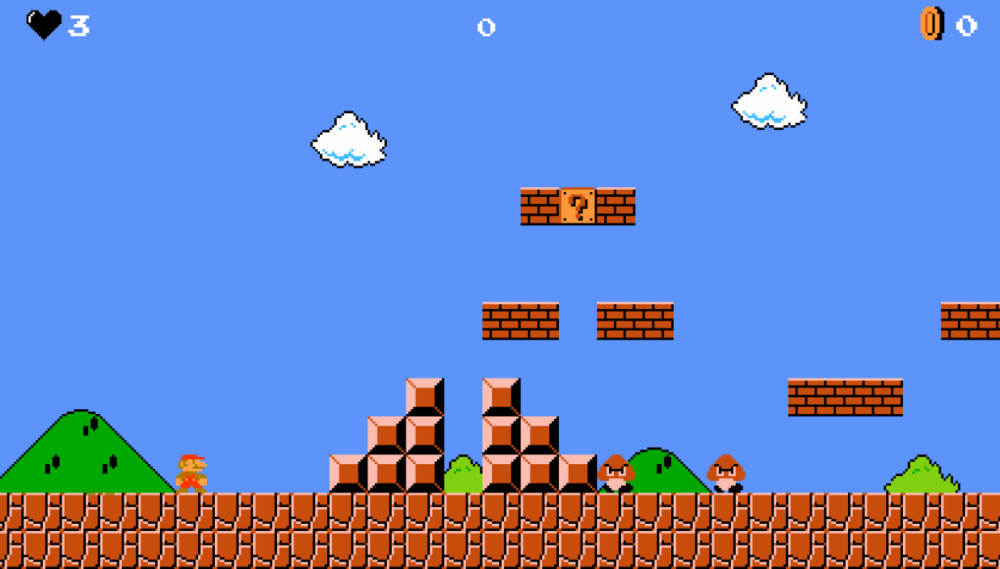
\includegraphics[width=\linewidth]{figs/mario-screenshot.png}
   \end{columns}
\end{frame}

\subsection{Spritesheets}

\begin{frame}{Sprites}{Spritesheets}
    \begin{columns}
 	   \column{.50\textwidth}
    A videogame contains many sprites
        \begin{itemize}
        \item Difficult maintenance
        \item Solution: Spritesheets
	    \end{itemize}

 	   \column{.50\textwidth}
    Advantages
        \begin{itemize}
        \item One file contains many sprites
        \item Less I/O operations $\Rightarrow$ Better performance
        \item Less memory consumption
	    \end{itemize}
   \end{columns}

    \centering

    \begin{columns}
 	   \column{.50\textwidth}
		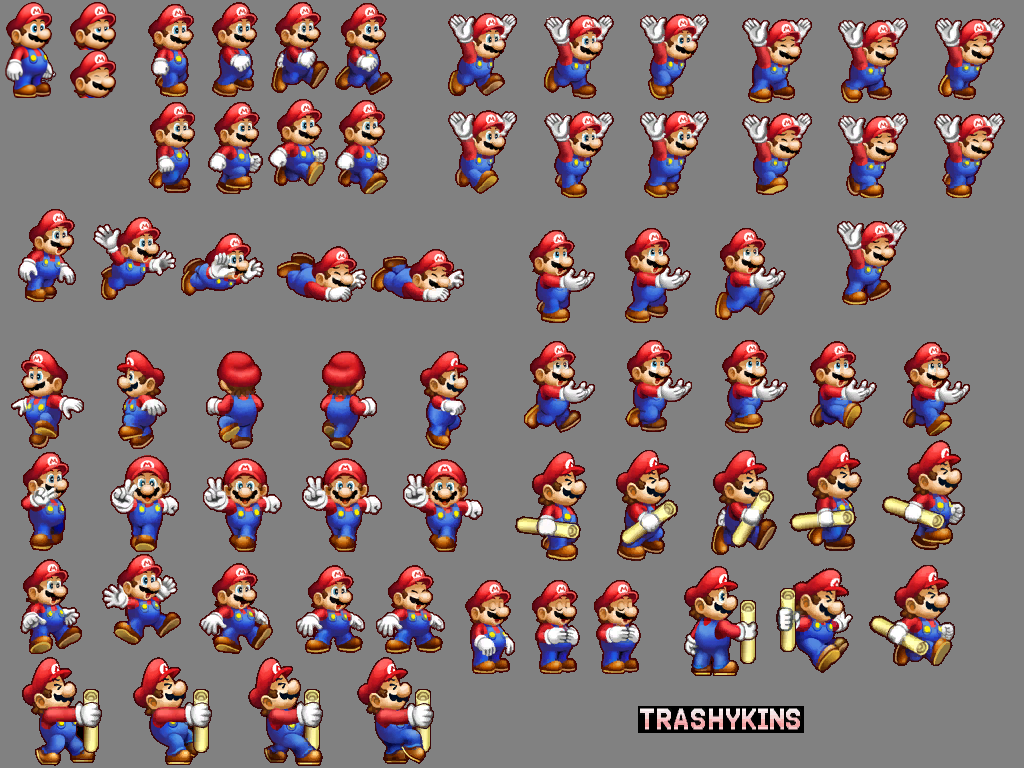
\includegraphics[width=\linewidth]{figs/mario-spritesheet.png}

 	   \column{.50\textwidth}
		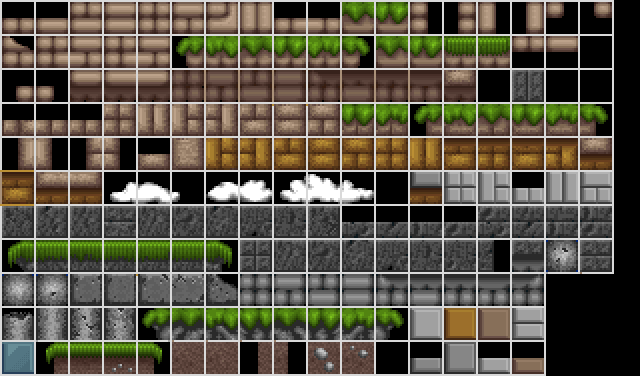
\includegraphics[width=\linewidth]{figs/blocks1.png}
   \end{columns}
\end{frame}

\subsection{Data formats}

\begin{frame}{Sprites}{Data formats (I)}
    In genenal, any data can be stored in three forms
        \begin{itemize}
        \item Not compressed
        \item Compressed with loss
        \item Compressed without loss
	    \end{itemize}

    \begin{table}
    \centering
    \begin{tabular}{l|c|c|c}
                            & Image format & Sound format & Binary data\\\hline
    Not compressed          & BMP          & WAV  &  \\
    Compressed with loss    & JPG          & MP3  &  \\
    Compressed without loss & PNG, GIF     & -    & ZIP, bzip, rar, ... 
    \end{tabular}
    \end{table}
\end{frame}

\begin{frame}{Sprites}{Data formats (II)}
    Attending to what information is stored in image format, there are two types of image formats:
        \begin{itemize}
            \item Bitmap: stores each pixel
                \begin{itemize}
                \item Scales bad
                \item Formats: JPG, PNG, BMP, GIF
                \end{itemize}

            \item Vectorial: stores coordinates
                \begin{itemize}
                \item Scales well
                \item Not supported by Arcade
                \item Formats: SVG, EPS
                \end{itemize}
	    \end{itemize}

    Many open assets for your games!
        \begin{itemize}
        \item \href{https://kenney.nl/assets}{(Kenney)}
        \end{itemize}
\end{frame}

\subsection{The \texttt{Sprite} class}

\begin{frame}{Sprites}{The \texttt{Sprite} class (I)}
    You will need to provide a \alert{path} to the file
    \begin{itemize}
        \item \textit{Absolute path}: Starts from the root directory
            \begin{itemize}
            \item Example (Windows): \texttt{c:\textbackslash\textbackslash Users\textbackslash atreides\textbackslash Desktop\textbackslash mygame\textbackslash assets\textbackslash sprites\textbackslash mario.png}
            \item Example (Linux): \texttt{/home/atreides/mygame/assets/sprites/mario.png}
            \end{itemize}
        \item \textit{Relative path}: Relative to the project's directory
            \begin{itemize}
            \item Example (Windows): \texttt{assets\textbackslash sprites\textbackslash mario.png}
            \item Example (linux): \texttt{assets/sprites/mario.png}
            \end{itemize}
    \end{itemize}

    \textbf{Always} use relative paths in your projects!!!
\end{frame}

\begin{frame}{Sprites}{The \texttt{Sprite} class (II)}
	Sprites are a fundamental concept in Arcade
    
    \begin{columns}
 	   \column{\textwidth}
		\begin{exampleblock}{Creating a sprite}
        \texttt{
        character = arcade.Sprite('images/character.png')
        }
		\end{exampleblock}
    \end{columns}

    \begin{columns}
 	   \column{.50\textwidth}
		\begin{exampleblock}{Placing a sprite}
        \texttt{
        character.center\_x = 300\\
        character.center\_y = 200}
		\end{exampleblock}

    \end{columns}
\end{frame}

\begin{frame}{Sprite}{The \texttt{Sprite} class (III)}
	\href{https://api.arcade.academy/en/latest/api/sprites.html}{(Reference documentation)}

	\begin{block}{Constructor}
		\vspace{-0.2cm}
		\lstinputlisting{code/sprite-init.py}
		\vspace{-0.2cm}
	\end{block}	

\end{frame}

\begin{frame}{Sprite}{The \texttt{Sprite} class (IV)}
    Sprites in Arcade implement \alert{collision detection} and handling

	\begin{columns}
 	   \column{.5\textwidth}
		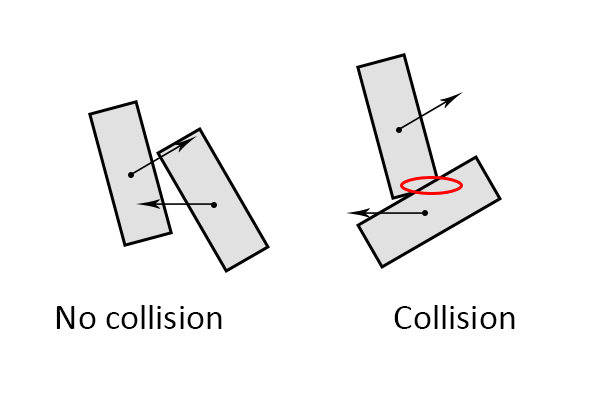
\includegraphics[width=\linewidth]{figs/collision}\\
		%\vspace{-0.3cm}\tiny \href{https://stackoverflow.com/questions/46268139/2d-collision-detection-without-axis-alignment}{(Source)}
	\end{columns}

 

    Three values for \texttt{hit\_box\_algoritm}: `None`, `Simple` and `Detailed`

    \begin{columns}
 	   \column{.3\textwidth}
		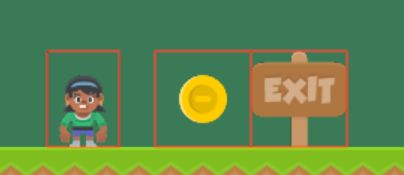
\includegraphics[width=\linewidth]{figs/hitbox-none}\\
		\centering None'
	   \column{.3\textwidth}
		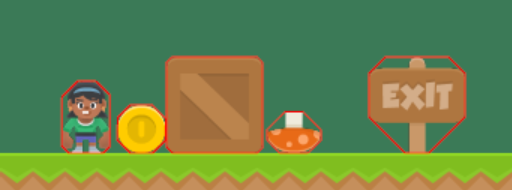
\includegraphics[width=\linewidth]{figs/hitbox-simple}\\
		\centering 'Simple'
	   \column{.3\textwidth}
		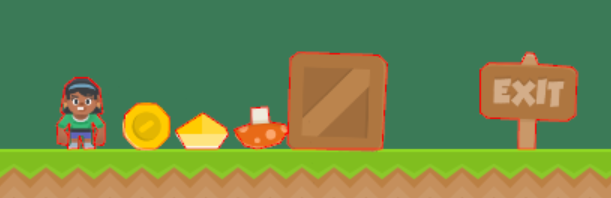
\includegraphics[width=\linewidth]{figs/hitbox-detailed}\\
		\centering 'Detailed'
    \end{columns}
\end{frame}

\begin{frame}[plain]{Sprite}{The \texttt{Sprite} class (V)}
	\begin{block}{\texttt{arcade.Sprite}}
		\smallskip
		\begin{columns}[t]
 	   \column{.5\textwidth}
			\centering \textbf{Methods}
		\begin{itemize}
		\item \footnotesize{\texttt{on\_update(delta\_time: float = 0.016)}}. 
		\item \footnotesize{\texttt{draw()}}. 
		\item \footnotesize{\texttt{append\_texture(Texture: arcade.texture.Texture}}. \\ Appends a new texture (image)
		\item \footnotesize{\texttt{set\_texture(texture\_no: int)}}. \\
		\item \footnotesize{\texttt{update\_animation(delta\_time: float = 0.016))}}. \\
		\item \footnotesize{\texttt{set\_position(center\_x: float, center\_y: float)}}. \\
		\item \footnotesize{\texttt{turn\_left(theta: float = 90.0)}} 
		\item \footnotesize{\texttt{turn\_right(theta: float = 90.0)}} 
		\item \footnotesize{\texttt{stop()}} 
		\end{itemize}

 	   \column{.5\textwidth}
			\centering \textbf{Attributes}
		\begin{itemize}
		\item \footnotesize{alpha: int}.
		\item \footnotesize{angle: float}. 
		\item \footnotesize{bottom: float} and \footnotesize{bottom: float}. 
		\item \footnotesize{center\_x: float} and \footnotesize{center\_y: float}.\\ Center of the sprite
		\item \footnotesize{change\_x: float} and \footnotesize{change\_y: float}.\\ Velocity in X and Y
		\item \footnotesize{height: float}. 
		\item \footnotesize{visible: bool}. 
		\end{itemize}
			\vfill
	    \href{https://api.arcade.academy/en/2.6.17/api/sprites.html\#arcade-sprite}{(Reference documentation)}
    	\end{columns}
	\end{block}	

\end{frame}

\subsection{Examples}

\begin{frame}[fragile]{Sprites}{The \texttt{Sprite} class: Examples}
	\begin{exampleblock}{}
	\lstinputlisting[numbers=left]{code/visible.py}
	\end{exampleblock}
\end{frame}

\subsection{Collision detection}

\begin{frame}{Sprites}{Collision detection}
	\begin{block}{Collision detection methods}
	%	\vspace{-0.15cm}
		\begin{itemize}
		\item \footnotesize{\texttt{collides\_with\_point(point: Union[Tuple[float, float], List[float]]) $\rightarrow$ bool}} 
		\item \footnotesize{\texttt{draw\_hit\_box()}}. 
		\item \footnotesize{\texttt{collides\_with\_list(sprite\_list: SpriteList) $\rightarrow$ bool}} 
		\end{itemize}
	%	\vspace{-0.2cm}
	\end{block}	
\end{frame}

\subsection{Other classes}

\begin{frame}[fragile]{Sprite}{Other classes}
	\begin{tikzpicture}
      \begin{class}[text width=4cm]{Sprite}{0,0}
      \end{class}

      \begin{class}[text width=3cm]{SpriteCircle}{-4,-2}
	\inherit{Sprite}
      \end{class}

	\begin{class}[text width=3cm]{SpriteSolidColor}{0,-2}
	\inherit{Sprite}
      \end{class}

       \begin{class}[text width=4cm]{AnimatedTimeBasedSprite}{4, -2}
	\inherit{Sprite}
      \end{class}
    \end{tikzpicture}
	\begin{itemize}
		\item \href{https://api.arcade.academy/en/2.6.17/api/sprites.html\#arcade-spritecircle}{(SpriteCircle documentation)}
		\item \href{https://api.arcade.academy/en/2.6.17/api/sprites.html\#arcade-spritesolidcolor}{(SpriteSolidColor documentation)}
		\item \href{https://api.arcade.academy/en/2.6.17/api/sprites.html\#arcade-animatedtimebasedsprite}{(SpriteAnimatedTimeBasedSprite documentation)}
	\end{itemize}
\end{frame}

\subsection{Sprite lists}

\begin{frame}{Sprites}{Sprite lists (I)}
	Arcade stores sprites in lists
    
	\begin{exampleblock}{}
	\lstinputlisting{code/lists.py}
	\end{exampleblock}

       Lists can be manipulated as a whole

	\begin{exampleblock}{}
        \texttt{
        wall\_list.draw()
        }
	\end{exampleblock}

    	And sprites can be removed from a list
	\begin{exampleblock}{}
        \texttt{
        wall.remove\_from\_sprite\_lists()
        }
	\end{exampleblock}
\end{frame}

\begin{frame}{Sprites}{Sprite lists (II)}
    Lists in Arcade also implement collision detection 
	\begin{exampleblock}{}
        \texttt{
            hit\_list = arcade.check\_for\_collision\_with\_list(player\_sprite,
                                                              coin\_list)
        }
    \end{exampleblock}

    Functional example in \href{https://gist.github.com/dfbarrero/83294a5ea218ca866b68558d4d64ba46}{(example)}
\end{frame}

\subsection{Locating sprites}

\begin{frame}{Sprites}{Locating sprites}
    Locating sprites in the game is a tought work
    \begin{itemize}
        \item Closely related to \alert{level design}
        \item There are tools that ease this task
    \end{itemize}
    \href{https://www.mapeditor.org/}{(Tiled Map Editor)}

	\vspace{-2.5cm}
    \hfill 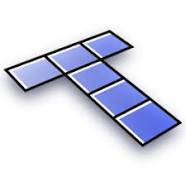
\includegraphics[width=0.3\linewidth]{figs/tiled}
\end{frame}

\section{Resources management}

\begin{frame}{Resources management (I)}
    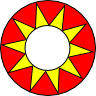
\includegraphics[width=0.07\linewidth]{figs/bumper}
    
\includegraphics[width=0.07\linewidth]{figs/laserBlue01}
    
\includegraphics[width=0.07\linewidth]{figs/tileGrass_roadSplitE}
    
\includegraphics[width=0.07\linewidth]{figs/coinGold_ul}
    \includegraphics[width=0.07\linewidth]{figs/frog\_move}
    
\includegraphics[width=0.07\linewidth]{figs/planet}
    \includegraphics[width=0.07\linewidth]{figs/stoneHill\_left}
    
\includegraphics[width=0.07\linewidth]{figs/water}
    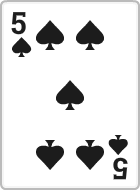
\includegraphics[width=0.07\linewidth]{figs/cardSpades5}
    
\includegraphics[width=0.07\linewidth]{figs/slimeBlue}
    \includegraphics[width=0.07\linewidth]{figs/femaleAdventurer\_walk3}
    \includegraphics[width=0.07\linewidth]{figs/zombie\_idle}

    \bigskip

    Arcade comes along a collection of built-in resources
    \begin{itemize}
        \item Good for testing
        \item No need of files in disk
	\item Images, music, sounds, tiled maps and video
    \end{itemize}
    The path is something like ':resources:/path/to/resource'

    \begin{exampleblock}{}
	    \texttt{ arcade.Sprite(":resources:images/items/coinGold.png") }
    \end{exampleblock}

    \href{https://api.arcade.academy/en/2.6.17/resources.html\?highlight=resources}{(List of resources)}\\
    \href{https://github.com/pythonarcade/arcade/tree/development/arcade/resources/assets}{(Arcade source code)}
\end{frame}

\begin{frame}{Resources management (II)}
	\begin{exampleblock}{Adding new resources handlers}
	\lstinputlisting[numbers=left]{code/resources-1.py}
	\end{exampleblock}

	\begin{exampleblock}{Using resources handlers}
	\lstinputlisting[numbers=left]{code/resources-2.py}
	\end{exampleblock}
\end{frame}

\end{document}
